\documentclass{article}
\usepackage[utf8]{inputenc}
\usepackage[T1]{fontenc}
\usepackage[polish]{babel}
\usepackage{graphicx}
\usepackage{booktabs}
\usepackage{float}

\usepackage[margin=2.5cm]{geometry}
\usepackage[utf8]{inputenc}   % kodowanie znaków UTF-8
\usepackage[T1]{fontenc}      % poprawne kodowanie fontów
\usepackage[polish]{babel}    % język dokumentu: polski

\title{Dokumentacja Projektu}
\author{Piotr Ratajczak \and Alekasander Staszewski \and Wojciech Tomaszewski \and Krzysztof Zaporowski}
\date{\today}

\begin{document}

\maketitle

\section{Wprowadzenie i specyfikacja wymagań}
\subsection{Cel projektu}
Celem projektu jest stworzenie systemu robotycznego generującego iluzję optyczną poprzez wykorzystanie zjawiska 
Persistence of Vision (POV). System ma za zadanie wyświetlać tekst na obracającej się listwie

\subsection{Wymagania funkcjonalne}
\begin{itemize}
    \item Wyświetlanie tekstu 
    \item Precyzyjna synchronizacja wyświetlania diod LED z pozycją obrotową
    \item Stabilne utrzymanie iluzji optycznej
\end{itemize}

\subsection{Wymagania techniczne}
\begin{itemize}
    \item Silnik o odpowiednim momencie obrotowym
    \item Pasek LED NeoPixel o wysokiej częstotliwości odświeżania
    \item Czujnik Halla do precyzyjnego określania pozycji kątowej
    \item Mikrokontroler z wystarczającą mocą obliczeniową do obsługi diod LED
    \item Stabilna konstrukcja mechaniczna zapewniająca płynny ruch
\end{itemize}

\subsection{Ograniczenia i wymagania}
\begin{itemize}
    \item Minimalna prędkość obrotowa zapewniająca efekt POV
    \item Maksymalna masa komponentów na listwie
    \item Wymagana stabilność mechaniczna konstrukcji
    \item Odpowiednie zasilanie dla wszystkich komponentów
    \item Bezpieczeństwo użytkowania (ochrona przed dostępem do ruchomych części)
\end{itemize}

\subsection{Opis pomysłu rozwiązania systemu komputerowego}
System komputerowy składa się z mikrokontrolera ATtiny85, który pełni rolę głównego elementu sterującego. Jego zadaniem jest:
\begin{itemize}
    \item Synchronizacja wyświetlania diod LED z pozycją obrotową listwy
    \item Przetwarzanie sygnałów z czujnika Halla
    \item Generowanie odpowiednich sekwencji świetlnych na pasku NeoPixel
\end{itemize}

\section{Rozwiązania techniczne i opis konstrukcji}
System opiera się na precyzyjnej synchronizacji między komponentami:
\begin{itemize}
    \item Czujnik Halla wykrywa magnes zamontowany pod listwą, generując sygnał referencyjny dla każdego pełnego obrotu
    \item Mikrokontroler ATtiny85 wykorzystuje ten sygnał do synchronizacji wyświetlania diod LED
    \item Pasek NeoPixel, dzięki wysokiej częstotliwości odświeżania, tworzy płynny obraz
    \item Silnik krokowy zapewnia stałą prędkość obrotową, niezbędną dla stabilności iluzji
\end{itemize}

Techniczny aspekt iluzji optycznej:
\begin{itemize}
    \item Obraz jest generowany przez sekwencyjne włączanie diod LED w odpowiednich momentach obrotu
    \item Częstotliwość odświeżania diod jest dostosowana do prędkości obrotowej
    \item Precyzyjne obliczenia czasowe zapewniają prawidłowe wyświetlanie obrazu
    \item Efekt POV (Persistence of Vision) wykorzystuje bezwładność ludzkiego oka do tworzenia pozornie statycznego obrazu
\end{itemize}

% \subsection{Rysunki techniczne}
% % Tutaj umieść rysunki techniczne lub zdjęcia komputera i urządzenia z opisem

% \section{Schematy i opis}

% \subsection{Schemat ideowy}
% Tutaj umieść schemat ideowy z opisem

% todo
% \subsection{Schematy montażowe} 
% Tutaj umieść schematy montażowe lub zdjęcia z opisem:
% - komputer
% - mechanika
% - silniki
% - zasilanie
% - czujniki

\subsection{Rysunek płytki do trawienia}
\begin{figure}[ht!]
    \centering
    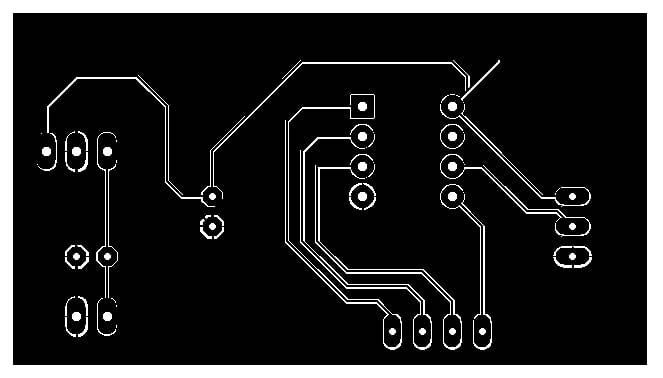
\includegraphics[width=0.8\textwidth]{plytka1.jpg}
    \label{fig:plytka1}
\end{figure}

\begin{figure}[ht!]
    \centering
    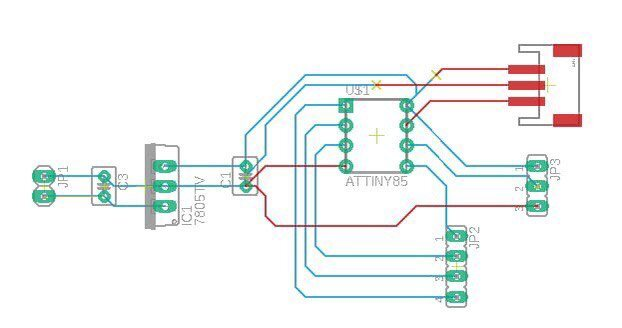
\includegraphics[width=0.8\textwidth]{plytka2.jpg}
    \label{fig:plytka2}
\end{figure}


\section{Oprogramowanie}
\subsection{Wykorzystane zasoby mikrokontrolera}
W projekcie wykorzystano następujące zasoby mikrokontrolera:
\begin{itemize}
    \item Pin cyfrowy 4 (DATA\_PIN) - do sterowania paskiem LED NeoPixel
    \item Pin cyfrowy 3 (SENSOR\_PIN) - do odczytu sygnału z czujnika Halla
    \item Pamięć RAM - do przechowywania bufora wyświetlania i danych fontu
    \item Pamięć Flash - do przechowywania programu i definicji znaków
    \item Timer - do precyzyjnego sterowania czasem wyświetlania
\end{itemize}

\subsection{Kod źródłowy}
\subsubsection{Algorytm}
Główny algorytm działania systemu opiera się na następujących elementach:
\begin{itemize}
    \item Synchronizacja z czujnikiem Halla w funkcji \texttt{loop()}
    \item Wyświetlanie tekstu poprzez sekwencyjne odświetlanie kolumn znaków
    \item Obsługa fontu 5x8 pikseli zdefiniowanego w tablicy \texttt{font[]}
\end{itemize}

\subsubsection{Obsługa przerwań}
System wykorzystuje przerwania do:
\begin{itemize}
    \item Wykrywania sygnału z czujnika Halla
    \item Synchronizacji wyświetlania z pozycją obrotową
    \item Precyzyjnego sterowania czasem świecenia diod LED
\end{itemize}

\subsubsection{Obsługa czujników}
\begin{itemize}
    \item Czujnik Halla podłączony do pinu 3
    \item Ciągłe monitorowanie stanu czujnika w pętli głównej
    \item Synchronizacja wyświetlania z każdym pełnym obrotem
\end{itemize}

\subsubsection{Obsługa elementów wykonawczych}
\begin{itemize}
    \item Sterowanie paskiem NeoPixel (8 diod) poprzez pin 4
    \item Biblioteka Adafruit\_NeoPixel do obsługi diod LED
    \item Precyzyjne sterowanie kolorem i jasnością diod
    \item Optymalizacja czasu odświeżania (750 mikrosekund na kolumnę)
\end{itemize}

\subsubsection{Przykładowy kod}
\begin{verbatim}
// Definicje pinów i parametrów
#define NUM_PIXELS  8      // Liczba diod LED w pasku
#define DATA_PIN    4      // Pin do sterowania paskiem LED
#define SENSOR_PIN  3      // Pin do odczytu czujnika Halla

// Zakres obsługiwanych znaków (tylko wielkie litery)
#define ASCII_START 'A'    // Pierwszy obsługiwany znak
#define ASCII_END   'Z'    // Ostatni obsługiwany znak

// Inicjalizacja paska LED NeoPixel
Adafruit_NeoPixel strip(NUM_PIXELS, DATA_PIN, NEO_GRB + NEO_KHZ800);

// Parametry fontu
const int charHeight = 8;  // Wysokość znaku w pikselach
const int charWidth = 5;   // Szerokość znaku w pikselach

// Funkcja inicjalizująca
void setup() {
    pinMode(SENSOR_PIN, INPUT);    // Konfiguracja pinu czujnika jako wejście
    strip.begin();                 // Inicjalizacja paska LED
    strip.show();                  // Wyłączenie wszystkich diod
}

// Główna pętla programu
void loop() {
    // Oczekiwanie na sygnał z czujnika Halla
    while (digitalRead(SENSOR_PIN) != HIGH) {
        strip.clear();             // Czyszczenie bufora diod
        strip.show();              // Aktualizacja stanu diod
    }
    displayText("HELLO");          // Wyświetlenie tekstu
}

// Funkcja wyświetlająca tekst
void displayText(const char* text) {
    for (int i = 0; i < strlen(text); i++) {
        char ch = text[i];
        // Sprawdzenie czy znak jest w obsługiwanym zakresie
        if (ch >= ASCII_START && ch <= ASCII_END) {
            // Wyświetlenie każdej kolumny znaku
            for (int j = 0; j < charWidth; j++) {
                displayColumn(font[ch - ASCII_START][j]);
            }
            displayColumn(0x00);   // Dodanie odstępu między literami
        }
    }
}

// Funkcja wyświetlająca pojedynczą kolumnę znaku
void displayColumn(byte column, bool flipped = false) {
    strip.clear();                 // Czyszczenie bufora diod
    // Iteracja po wszystkich pikselach w kolumnie
    for (int i = 0; i < charHeight; i++) {
        // Odczyt stanu piksela (z uwzględnieniem odwrócenia)
        bool pixelOn = bitRead(column, flipped ? i : (7 - i));
        if (pixelOn) {
            // Ustawienie koloru diody (zielony)
            strip.setPixelColor(i, strip.Color(0, 150, 0));
        }
    }
    strip.show();                  // Aktualizacja stanu diod
    delayMicroseconds(750);        // Opóźnienie dla stabilności wyświetlania
}
\end{verbatim}

\section{Kosztorys}
\begin{table}[H]
\centering
\begin{tabular}{lccc}
\toprule
Część & Ilość sztuk & Miejsce zakupu & Cena \\
\midrule
Silnik RS-550 & 1 & Amazon & 25.26 zł \\
Kondensator 0.33nF & 1 & Zasoby własne & 0.00 zł \\
Kondensator 0.1mF & 1 & Zasoby własne & 0.00 zł \\
Włącznik przelotowy & 1 & Botland & 9.40 zł \\
Czujnik Halla & 1 & Botland & 4.50 zł \\
Przewody & - & Zasoby własne & 0.00 zł \\
Łącznik wału silnika & 1 & Botland & 15.50 zł \\
Stabilizator napięcia L7805ABV & 1 & Botland & 1.90 zł \\
Mikrokontroler ATtiny85 & 1 & Botland & 19.90 zł \\
NeoPixel 8 & 1 & Botland & 14.90 zł \\
\bottomrule
\end{tabular}
\caption{Kosztorys projektu}
\end{table}

\end{document} 
